
\section{Procédure de la recherche documentaire} 
\label{sec:app/demarche}

Tout au long de notre projet, nous avons été amenés à nous documenter sur diverses thématiques nécessaires pour la réalisation de notre haut-parleur et la rédaction d'un rapport complet au sujet de celui-ci.
Ces recherches nous ont été indispensables pour remplir deux objectifs : premièrement, la fabrication et l'étude du fameux haut-parleur, ce qui nécessitait de maîtriser de nouvelles notions, principalement de physique; et deuxièmement, la rédaction d'un petit \og article \fg\ sur chacun des thèmes que nous avions choisi d'approfondir, à savoir les membranes-caissons et les filtres passe-bande (voir le \chapter ~\ref{Synthèse des recherches} p. \pageref{Synthèse des recherches}).
\newline

Pour commencer, comme nous en savions très peu sur les haut-parleurs, nous avons lu un maximum d’informations très générales sur le sujet, principalement sur des sites internet et dans des encyclopédies. Afin de trouver des articles, nous recherchions les mots-clefs \og haut-parleur \fg\ et \og loudspeaker \fg\ dans les moteurs de recherche et dans l'index des encyclopédies. 
Cette étape \og d'éclaireur \fg\ nous a permis d'avoir un bonne vue d’ensemble sur la composition et le fonctionnement d’un haut-parleur, mais également d'identifier les concepts de physique qui jouent un rôle important dans un haut-parleur.  


Ensuite, il nous a fallu étudier de plus près les concepts nouveaux que nous avions repéré lors de notre première recherche : l'électromagnétisme, l'électrodynamique, l’acoustique, les filtres passe-bande, les amplificateurs,... Comme les sources internet devenaient de moins en moins fiables sur ces sujets plus \og théoriques \fg\ et de physique plus poussée, nous nous sommes tournés vers des ouvrages plus sérieux, tels que des encyclopédies et des livres, ainsi que notre livre de référence de physique \cite{Pearson}\textbf{REF OU PAS ? pcq on ne l'a pas utilisé à un endroit précis} %mettre la REFERENCE  ?? ou pas?
qui nous a particulièrement aidé. Une fois la théorie comprise, nous pouvions la mettre en pratique lors du dimensionnement de notre électro-aimant et en analysant les propriétés de notre circuit électrique. 
\newline

À ce stade-ci, nous avions acquis une compréhension suffisante des différentes parties du haut-parleur et des thématiques qui y sont liées que pour pouvoir choisir de manière pertinente deux thèmes à développer dans notre rapport. Notre premier choix s'est  porté sur les caissons et membranes (leurs formes, dimensions, matériaux, propriétés, etc.) car ces informations nous serviraient explicitement pour la confection matérielle du haut-parleur. Le second thème que nous avons choisi est le filtre passe-bande, notamment car nous avions repéré dans un livre une méthode de résolution de circuits à filtre (R-L-C) innovante et concise que nous trouvions intéressante à exposer et à comparer avec celle vue en cours de physique. 

A partir de ces deux thèmes nous avons rédigé une liste de mots-clés qui s'y rapportaient (que vous trouverez dans la figure ~\ref{Schema mots-clefs}).


\begin{figure}[hb]
\begin{center}
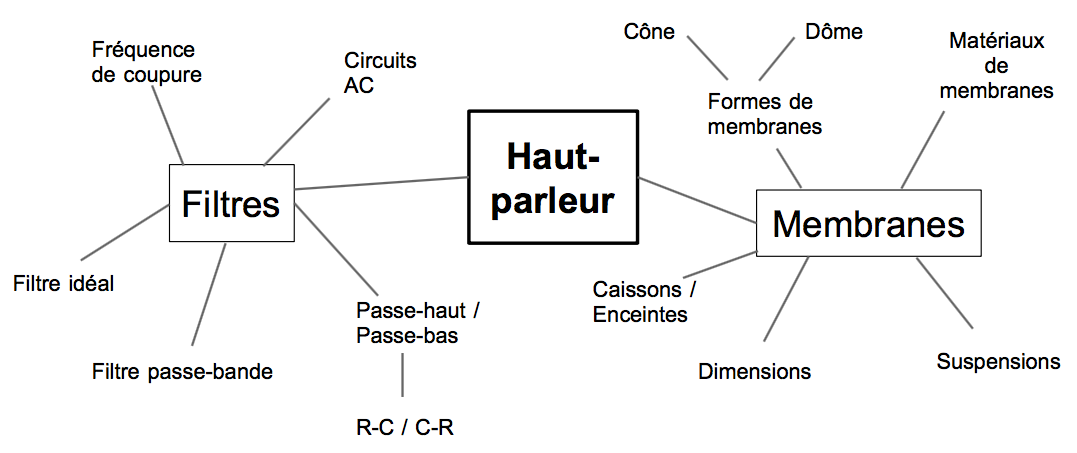
\includegraphics[scale=0.35]{img/Mots-clefs.png}
\end{center}
\caption{Schéma des mots-clés utilisés}
 \label{Schema mots-clefs}
\end{figure}


Nous nous en sommes servis pour rechercher dans l'index de livres, dans les moteurs de recherches pour trouver des brevets et sites fiables. Aussi bien en français qu'en anglais. Cette liste était régulièrement modifiée au cours de nos lectures. Pour la membrane, nous avons principalement récolté des brevets et des sites internet, tandis que pour les filtres, il s'agissait surtout de livres. 
Enfin, nous avons sélectionné parmi les nombreuses sources trouvées celles qui contenaient les informations nécessaires pour pouvoir rédiger un article sur les membranes et sur les filtres.
\newline

Ce travail nous a permis de nous rendre compte à quelle point la recherche documentaire est omniprésente dans tout travail scientifique pour acquérir les bases théoriques.
\newline


\section{Traces}

Les pages qui suivent contiennent les traces de certains extraits qui nous ont été utiles pour la synthèse de la recherche documentaire (voir figures : \ref{Trace 1}, \ref{Trace 2}, \ref{Trace 3}, \ref{Trace 4}, \ref{Trace 5}, \ref{Trace 6} et \ref{Trace 7}).

\begin{figure}
\begin{center}
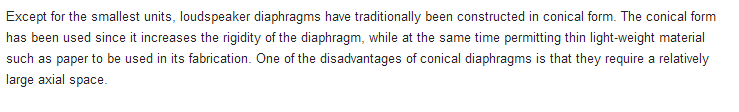
\includegraphics[scale=0.8]{img/Trace1-brevet US 3153463.png}
\end{center}
\caption{Extrait de \cite{f1964compound} \textbf{ICI Mettre auteur et titre et année?? ou pas?}} %REF bib
\label{Trace 1}
\end{figure}

\begin{figure}
\begin{center}
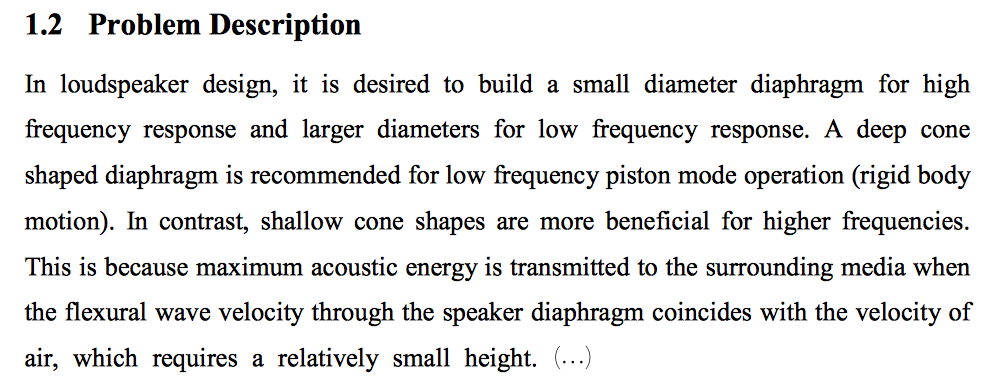
\includegraphics[scale=0.35]{img/Trace2-Miller.png}
\end{center}
\caption{Extrait de \cite[p.~2]{Miller} \textbf{ICI Mettre auteur et titre et année?? ou pas?}} %REF bib
\label{Trace 2}
\end{figure}

\begin{figure}
\begin{center}
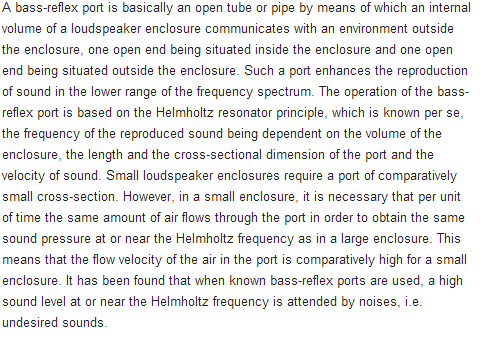
\includegraphics{img/Trace 3-US6275597.png}
\end{center}
\caption{Extrait de \cite{US6275597} \textbf{ICI Mettre auteur et titre et année?? ou pas?}} %REF bib
 \label{Trace 3}
\end{figure}

\begin{figure}
\begin{center}
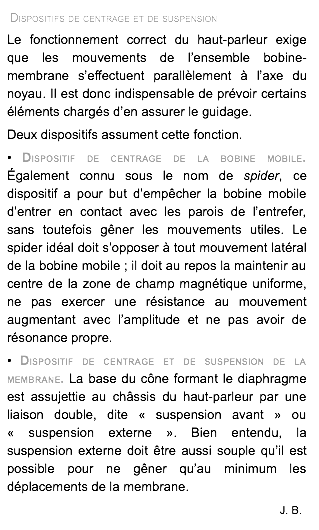
\includegraphics[scale = 0.5]{img/Larousse-1}
\end{center}
\caption{Extrait de \cite[p.~6486]{Larousse} \textbf{ICI Mettre auteur et titre et année?? ou pas?}} %REF bib
\label{Trace 4}
\end{figure}

\begin{figure}
\begin{center}
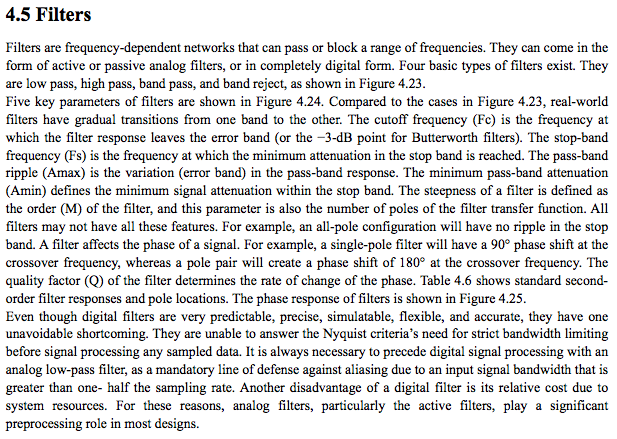
\includegraphics[scale=0.7]{img/Kularatna-1}
\end{center}
\caption{Extrait de \cite[p.~249-251]{Kularatna}\textbf{ICI Mettre auteur et titre et année?? ou pas?}} %REF bib
\label{Trace 5}
\end{figure}

\begin{figure}
\begin{center}
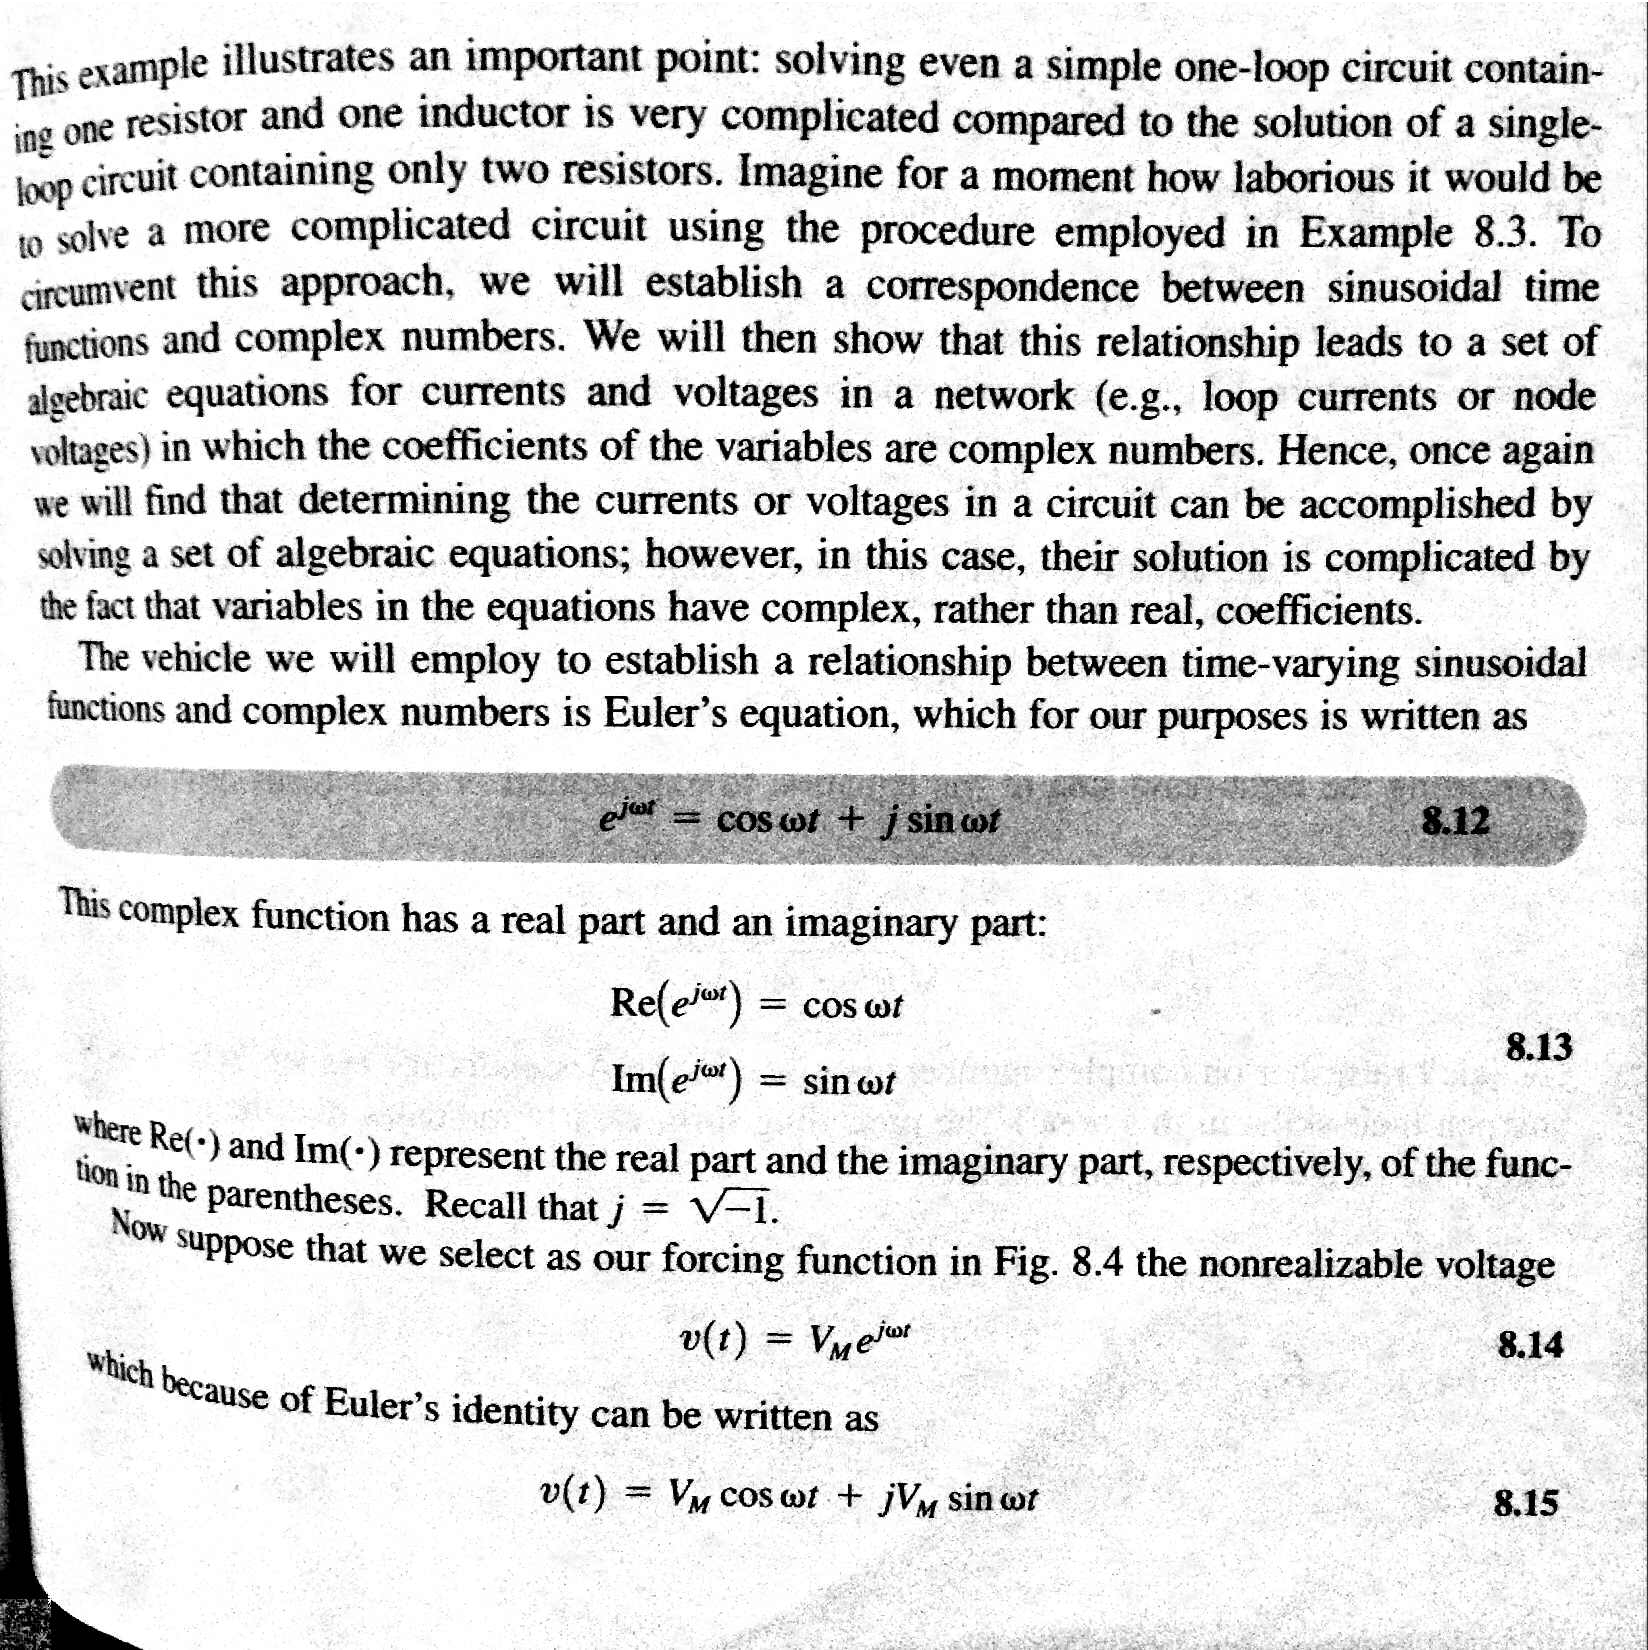
\includegraphics[scale=0.5]{img/Irwin-1}
\end{center}
\caption{Extrait de \cite[p.~375]{Irwin}\textbf{ICI Mettre auteur et titre et année?? ou pas?}}%REF bib 
\label{Trace 6}
\end{figure}

\begin{figure}
\begin{center}
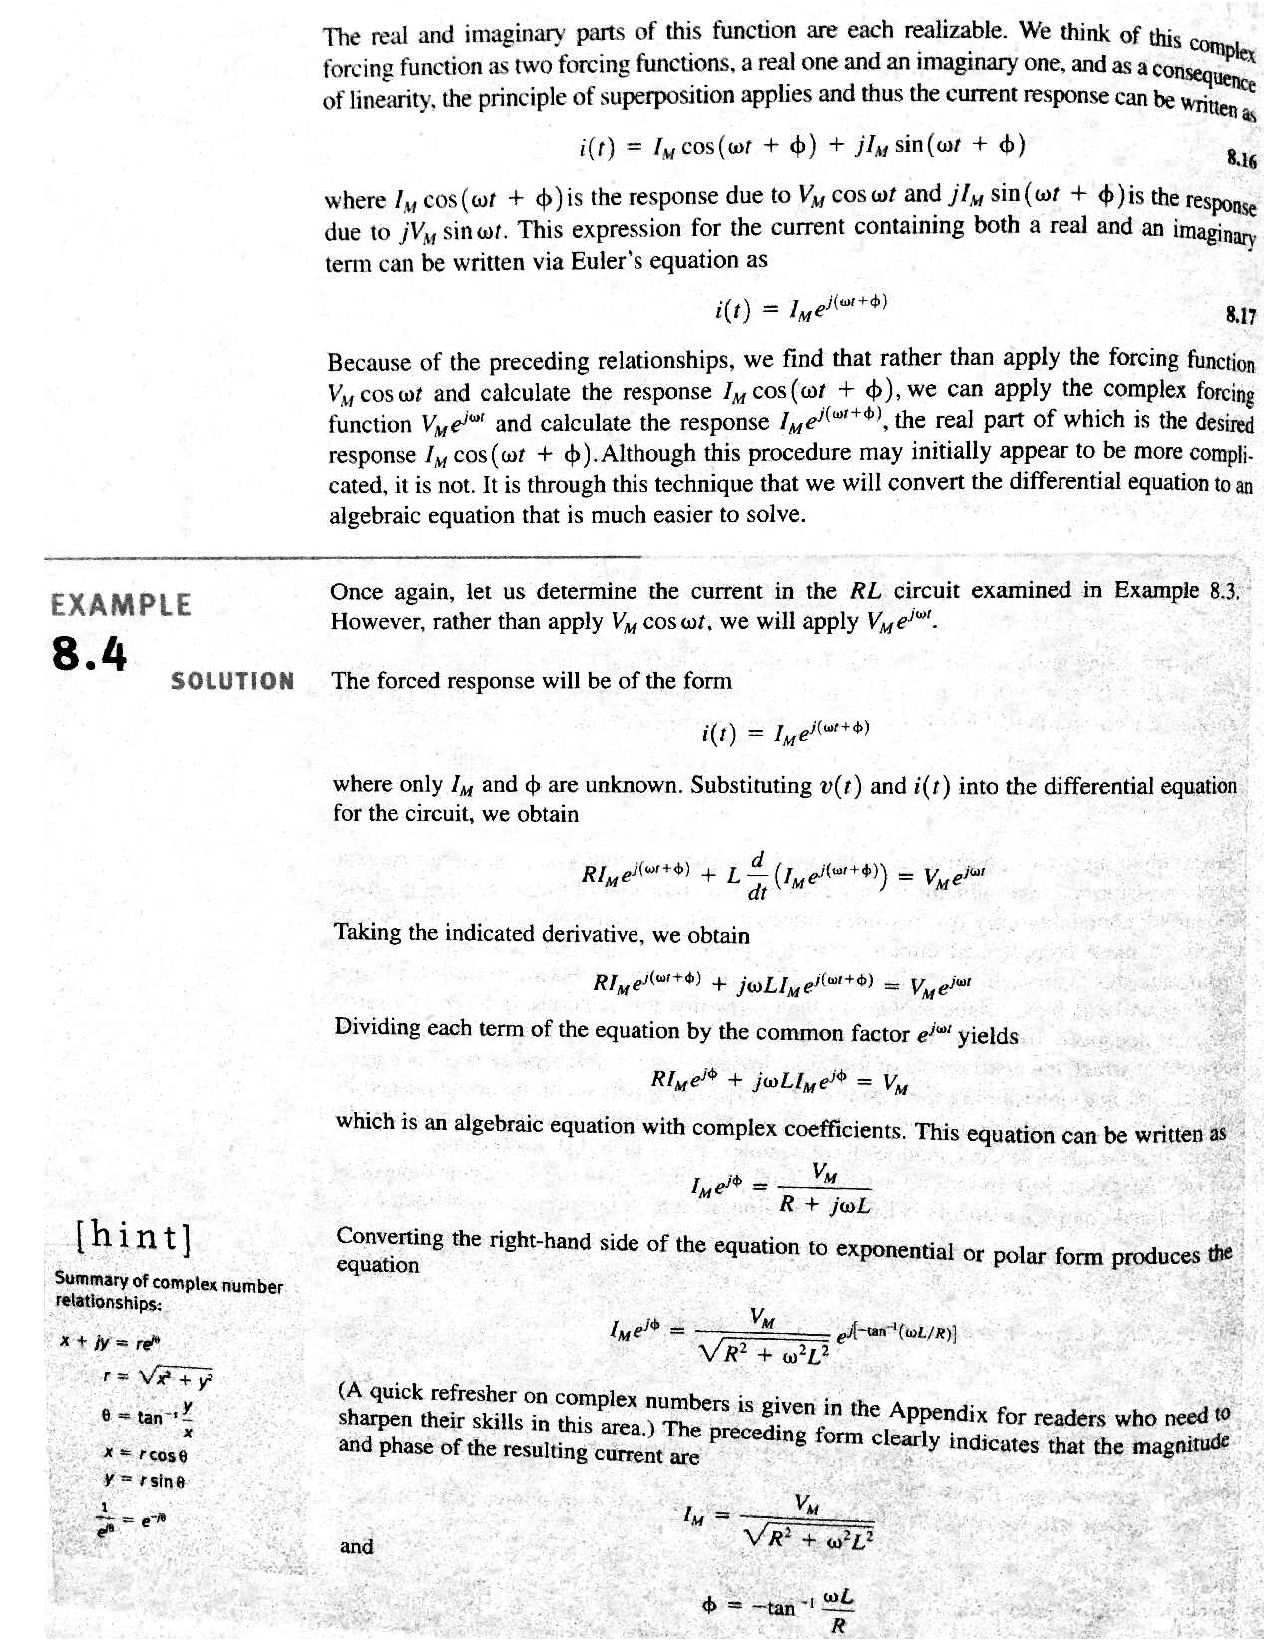
\includegraphics[scale=0.5]{img/Irwin-2} 
\end{center}
\caption{Extrait de \cite[p.~376]{Irwin}\textbf{ICI Mettre auteur et titre et année?? ou pas?}}%REF bib
\label{Trace 7}
\end{figure}


\

\

 
 
 
 
 


